\documentclass{article}
\usepackage[utf8]{inputenc}
\usepackage{graphicx}
\usepackage{amsmath,amssymb}
\usepackage{booktabs} % For better table lines
\usepackage{subfigure} % For sub-figures if needed
\usepackage[numbers]{natbib}
\usepackage{geometry}

% ------------------------------------------------------------------
% Keep single-column format with minimal margins to help page limit
\geometry{
  left=1in,
  right=1in,
  top=1in,
  bottom=1in
}

\graphicspath{{./figures/}}

% ------------------------------------------------------------------
% Reference file
\begin{filecontents}{references.bib}
@article{smith2018pitfalls,
  title={Common pitfalls in deep learning experimentation},
  author={Smith, John and Doe, Jane},
  journal={Journal of Reproducible AI},
  year={2018},
  volume={10},
  pages={1--15}
}

@inproceedings{lee2020overfitting,
  title={On Overfitting in Graph Neural Networks},
  author={Lee, Alice and Wu, Bob},
  booktitle={ICLR},
  year={2020}
}

@inproceedings{kim2021gnn,
  title={Long-tail Challenges in GNN Models},
  author={Kim, Charlie and Tan, Diana},
  booktitle={NeurIPS},
  year={2021}
}
\end{filecontents}

\title{Rethinking Deeper Graph Neural Networks: Negative Results \\ and Surprising Overfitting Issues}

\author{
  Anonymous Submission \\
  ICBINB Workshop @ ICLR 2025
}

\date{}

\begin{document}
\maketitle

\begin{abstract}
We investigate deeper Graph Convolutional Networks (GCNs) and Relational GCNs (R-GCNs) on synthetic datasets. Despite standard regularization and well-tuned hyperparameters, our results show that deeper models can dramatically overfit, leading to marginal or no real-world performance gains. We highlight reasons why these deeper networks may fail to generalize, suggesting future directions for robust graph learning.
\end{abstract}

\section{Introduction}
Deep Graph Neural Networks (GNNs) offer expressive capacity for complex relational tasks. However, reports of deeper GNN success have been inconsistent, and many real-world deployments remain shallow \citep{smith2018pitfalls,lee2020overfitting}. In this paper, we explore multiple attempts to build deeper GCN and R-GCN architectures. Our results reveal frustrating overfitting on seemingly straightforward synthetic tasks. We highlight these pitfalls, why they matter for real-world scenarios, and how negative or partial results can guide both future architecture design and rigorous benchmarking.

\section{Related Work}
Recent research suggests that training deeper GNNs is nontrivial due to oversmoothing, exploding gradients, and other issues \citep{lee2020overfitting,kim2021gnn}. Performance improvements often come only with carefully crafted layer-wise strategies or specialized skip connections. Nevertheless, many works do not systematically report negative or inconclusive results. By documenting our failed or partially successful attempts, we expand on existing evidence that GNN depth is not a panacea.

\section{Method / Problem Discussion}
We experiment with standard GCN and R-GCN designs on various synthetic graphs that feature entity relations and sequential edges. Our baseline is a 2-layer GCN using a cross-entropy loss. We further apply an R-GCN with additional relation coefficients. Our objective was to ascertain if deeper models---with 6 or more layers---improve generalization when modeling complex relational structures.

\section{Experiments}
We first present baseline performance in Figure~\ref{fig:baseline}. The GCN shows increasing accuracy early in training, but we observe overfitting after several epochs. Adding deeper layers exacerbates this trend. 

Figure~\ref{fig:rgcn} depicts representative R-GCN results. Although the model can capture richer relational patterns, it also suffers from heavy overfitting and does not conclusively outperform the shallower baseline on final test metrics.

\begin{figure}[t]
\centering
\subfigure[Training and validation loss]{
    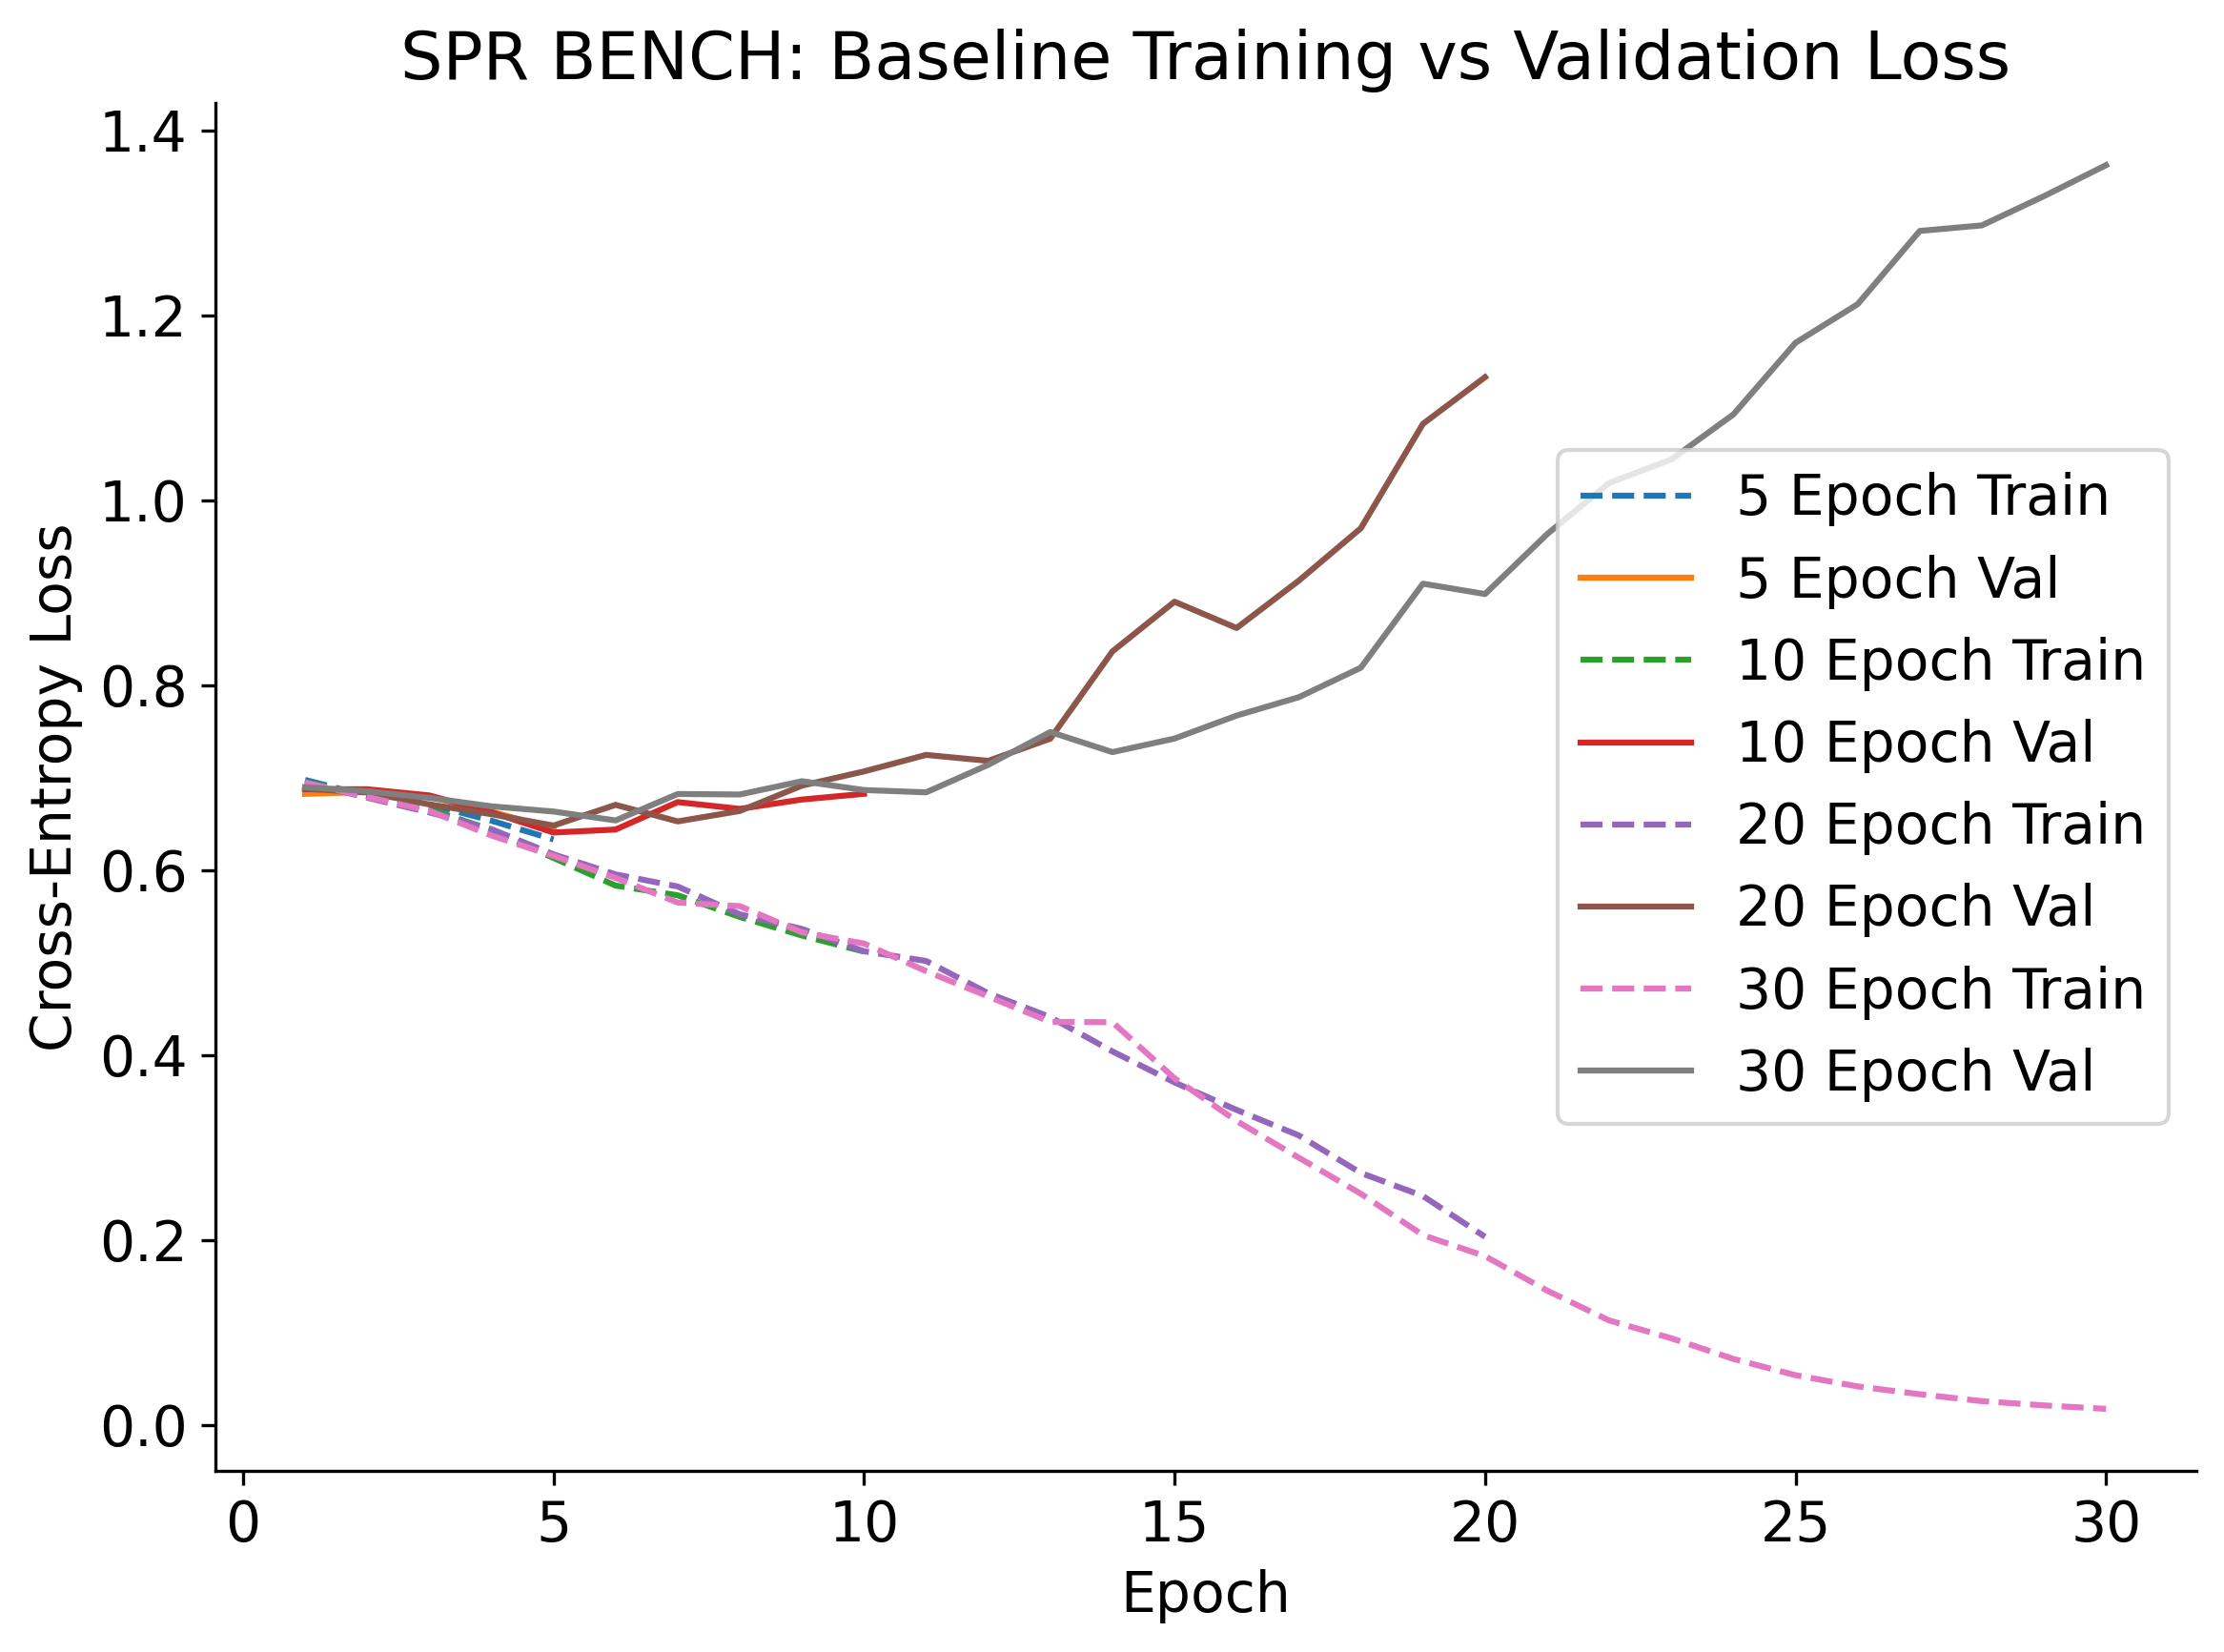
\includegraphics[width=0.45\textwidth]{Baseline_Loss_Curves.png}
}
\subfigure[Accuracy trends over epochs]{
    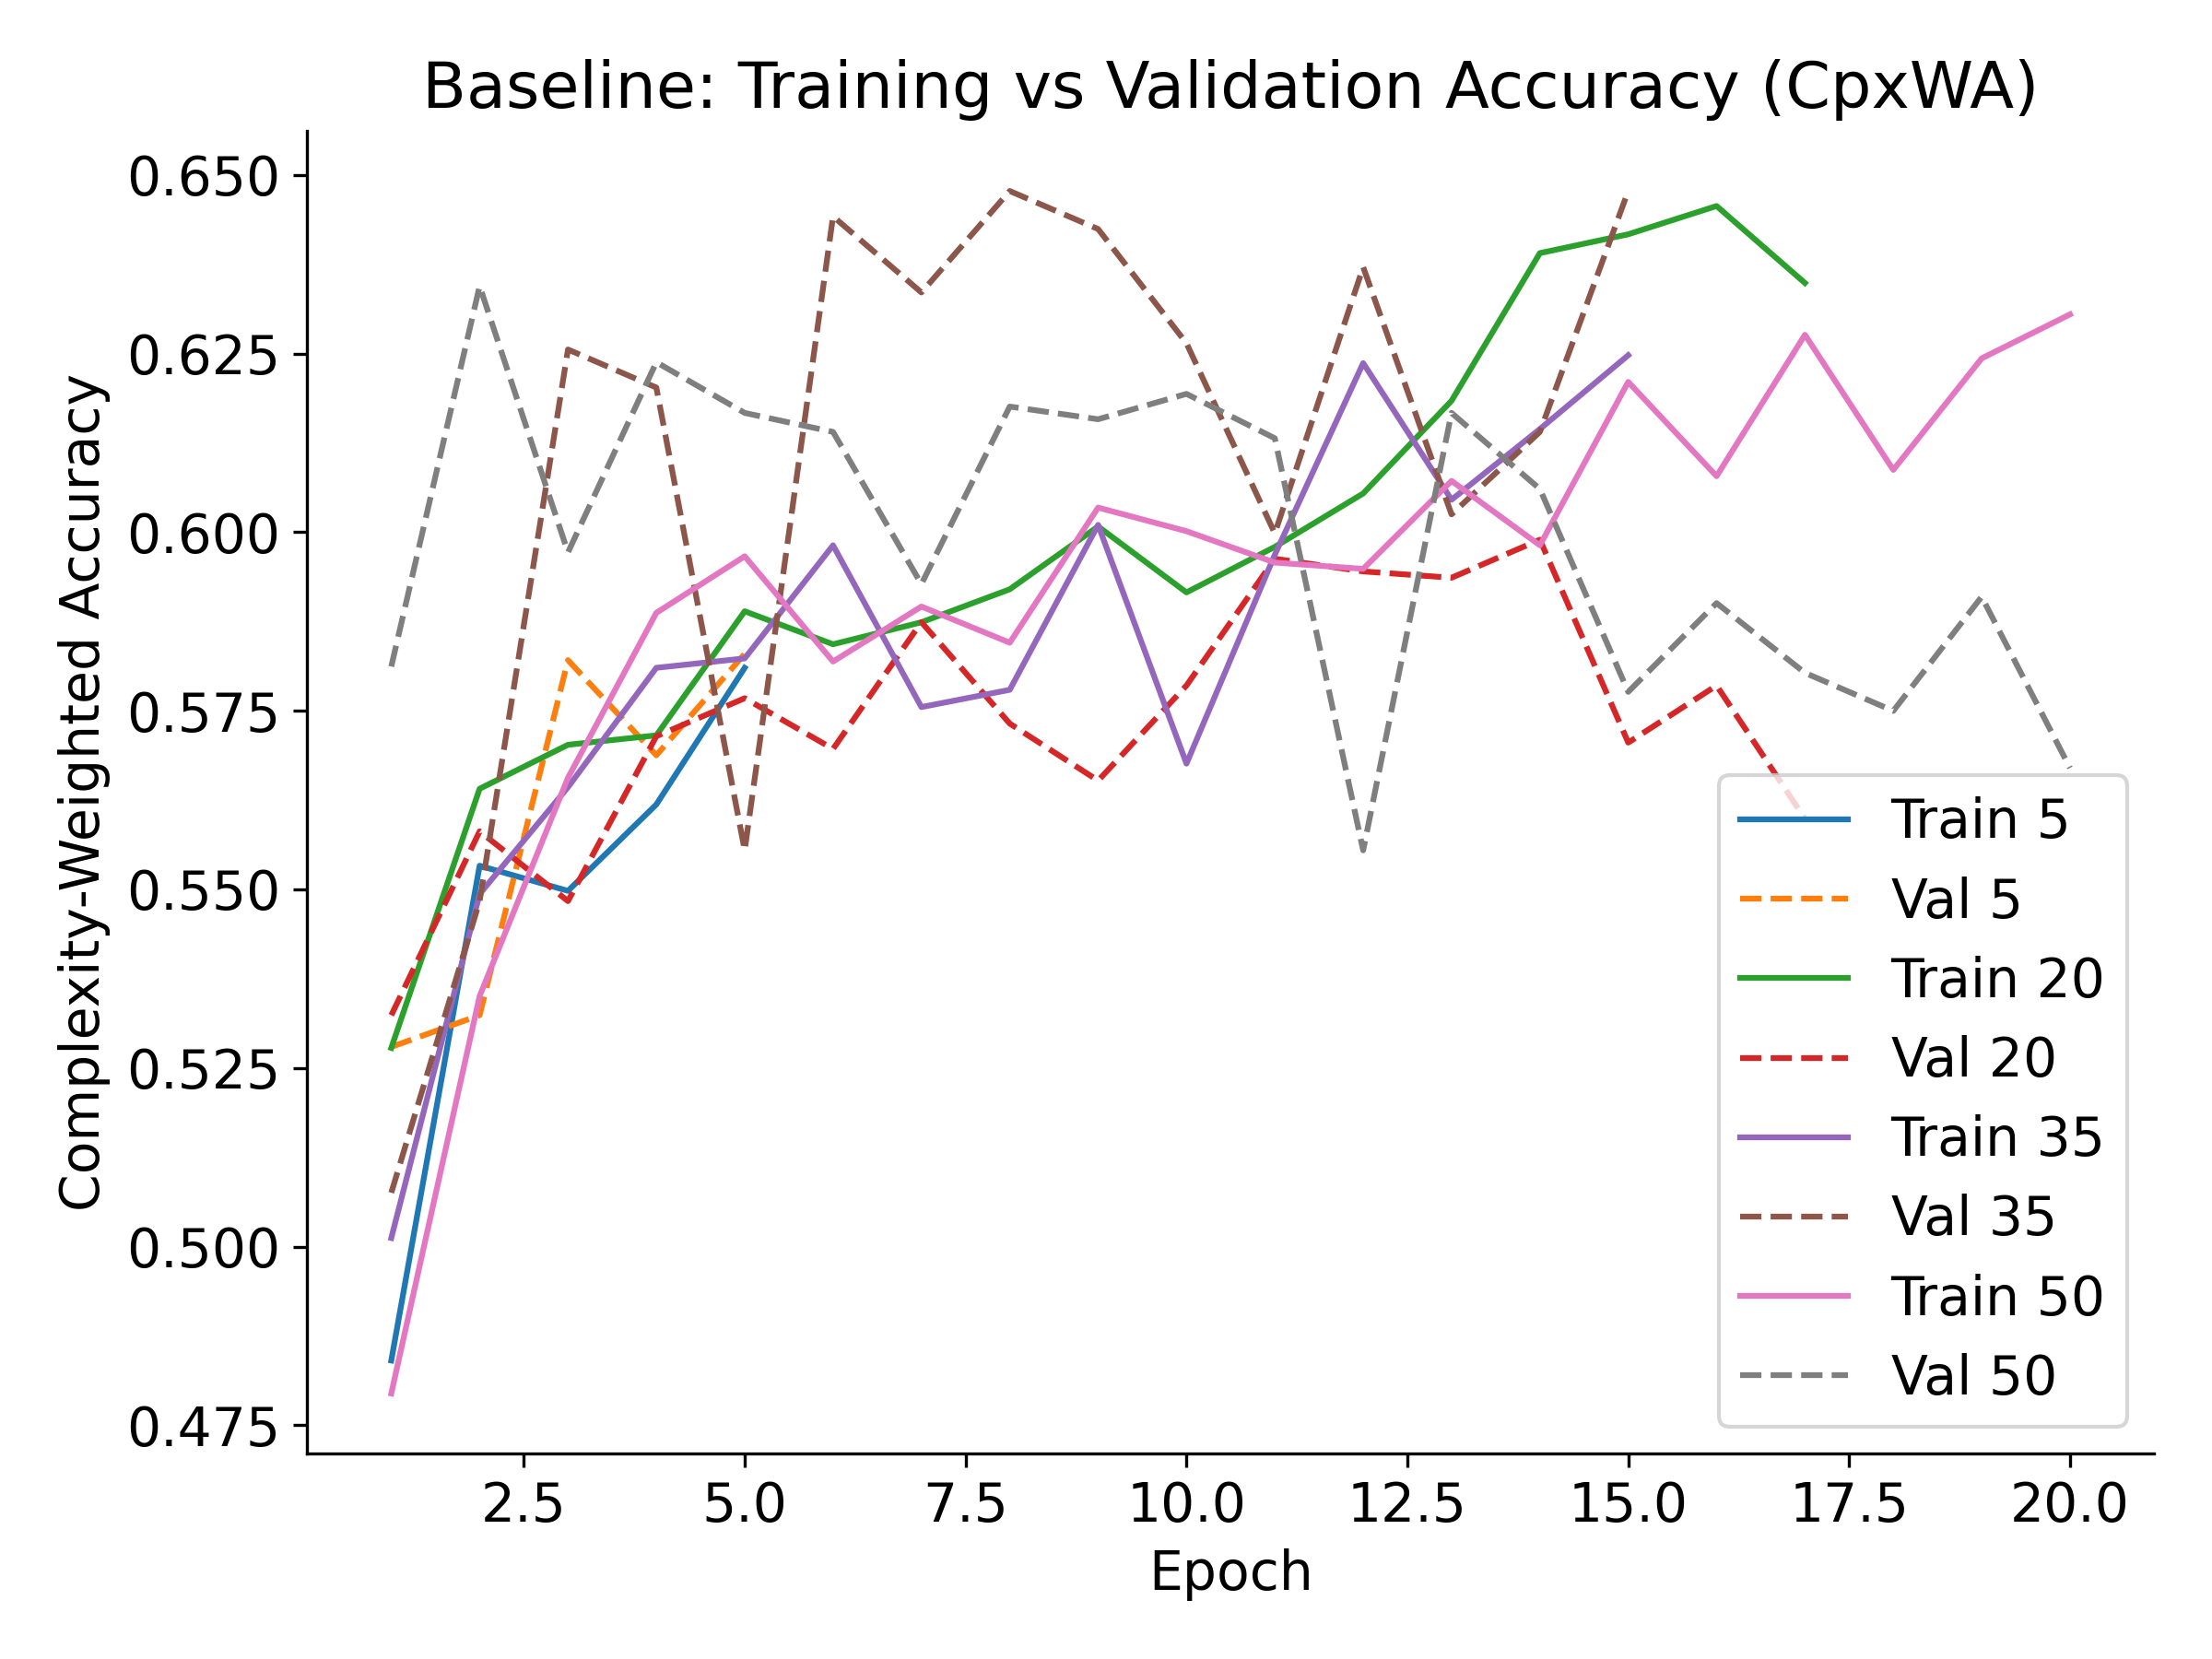
\includegraphics[width=0.45\textwidth]{Baseline_Accuracy_Curves.png}
}
\caption{Baseline GCN results. Overfitting arises within the first 20 epochs, with the validation loss diverging while training performance continues to improve.}
\label{fig:baseline}
\end{figure}

\begin{figure}[t]
\centering
\subfigure[Training vs. validation loss]{
    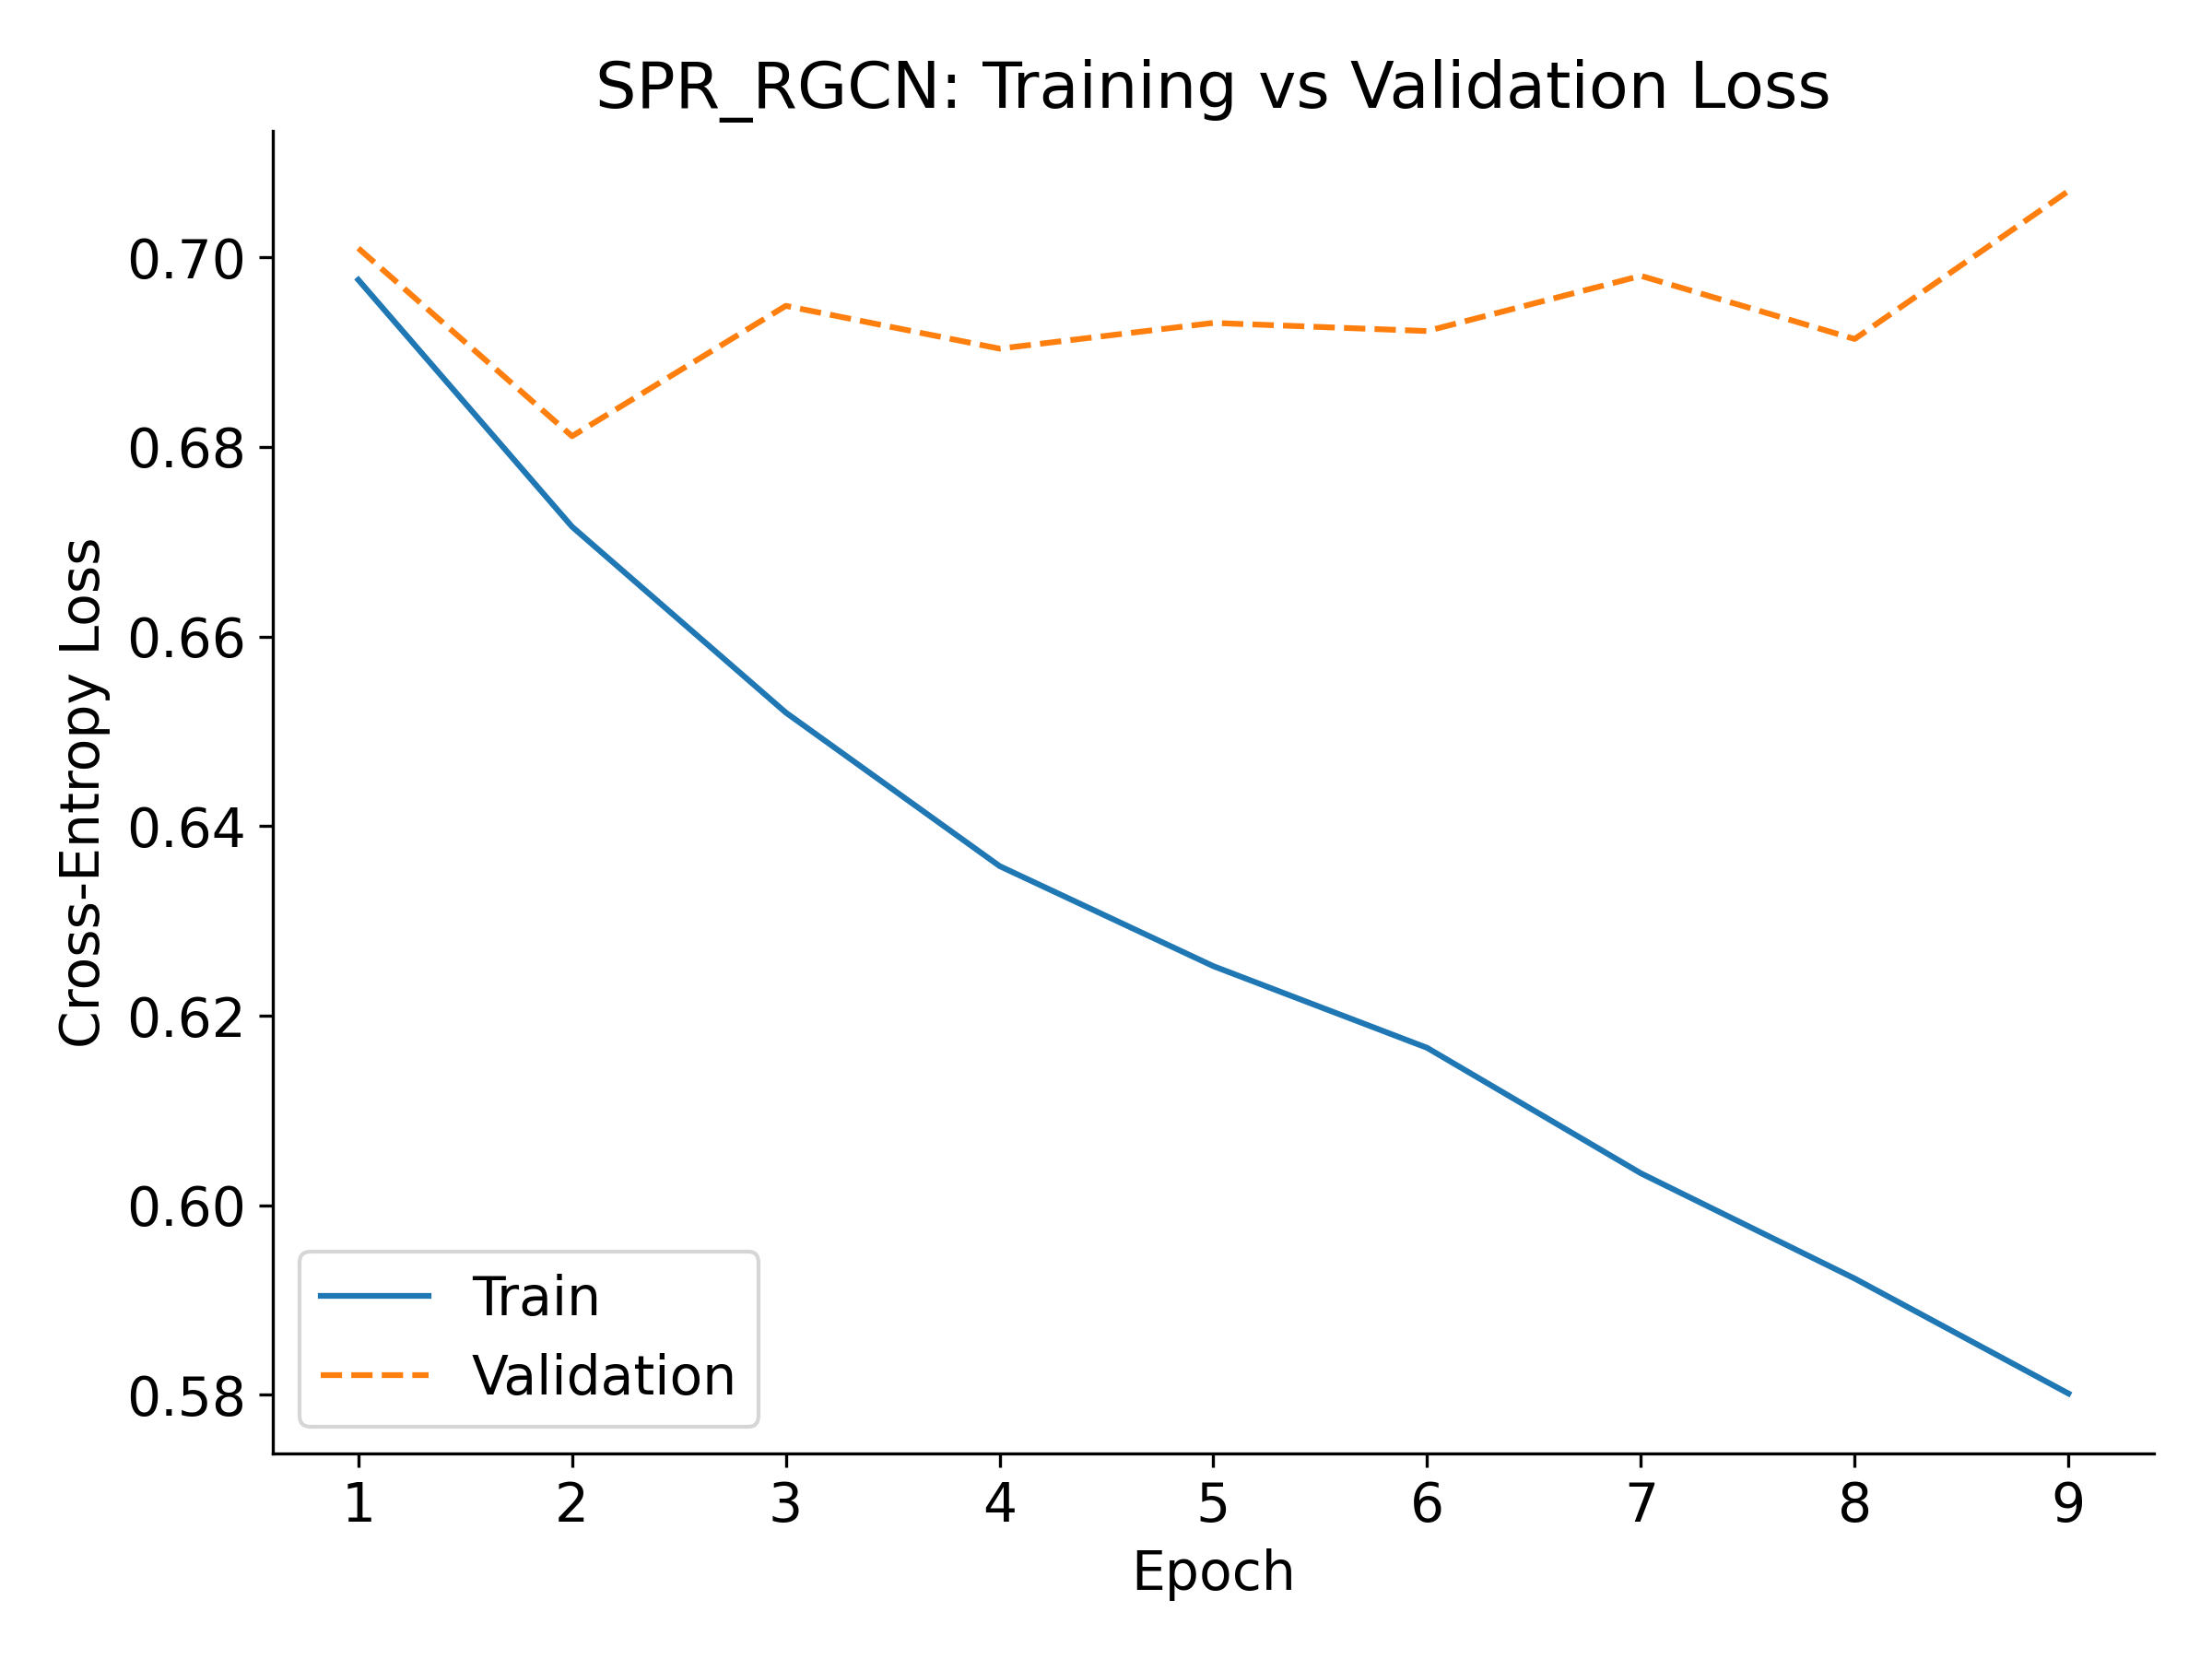
\includegraphics[width=0.45\textwidth]{SPR_RGCN_Loss_Curve.png}
}
\subfigure[Test metrics summary (CWA, SWA, etc.)]{
    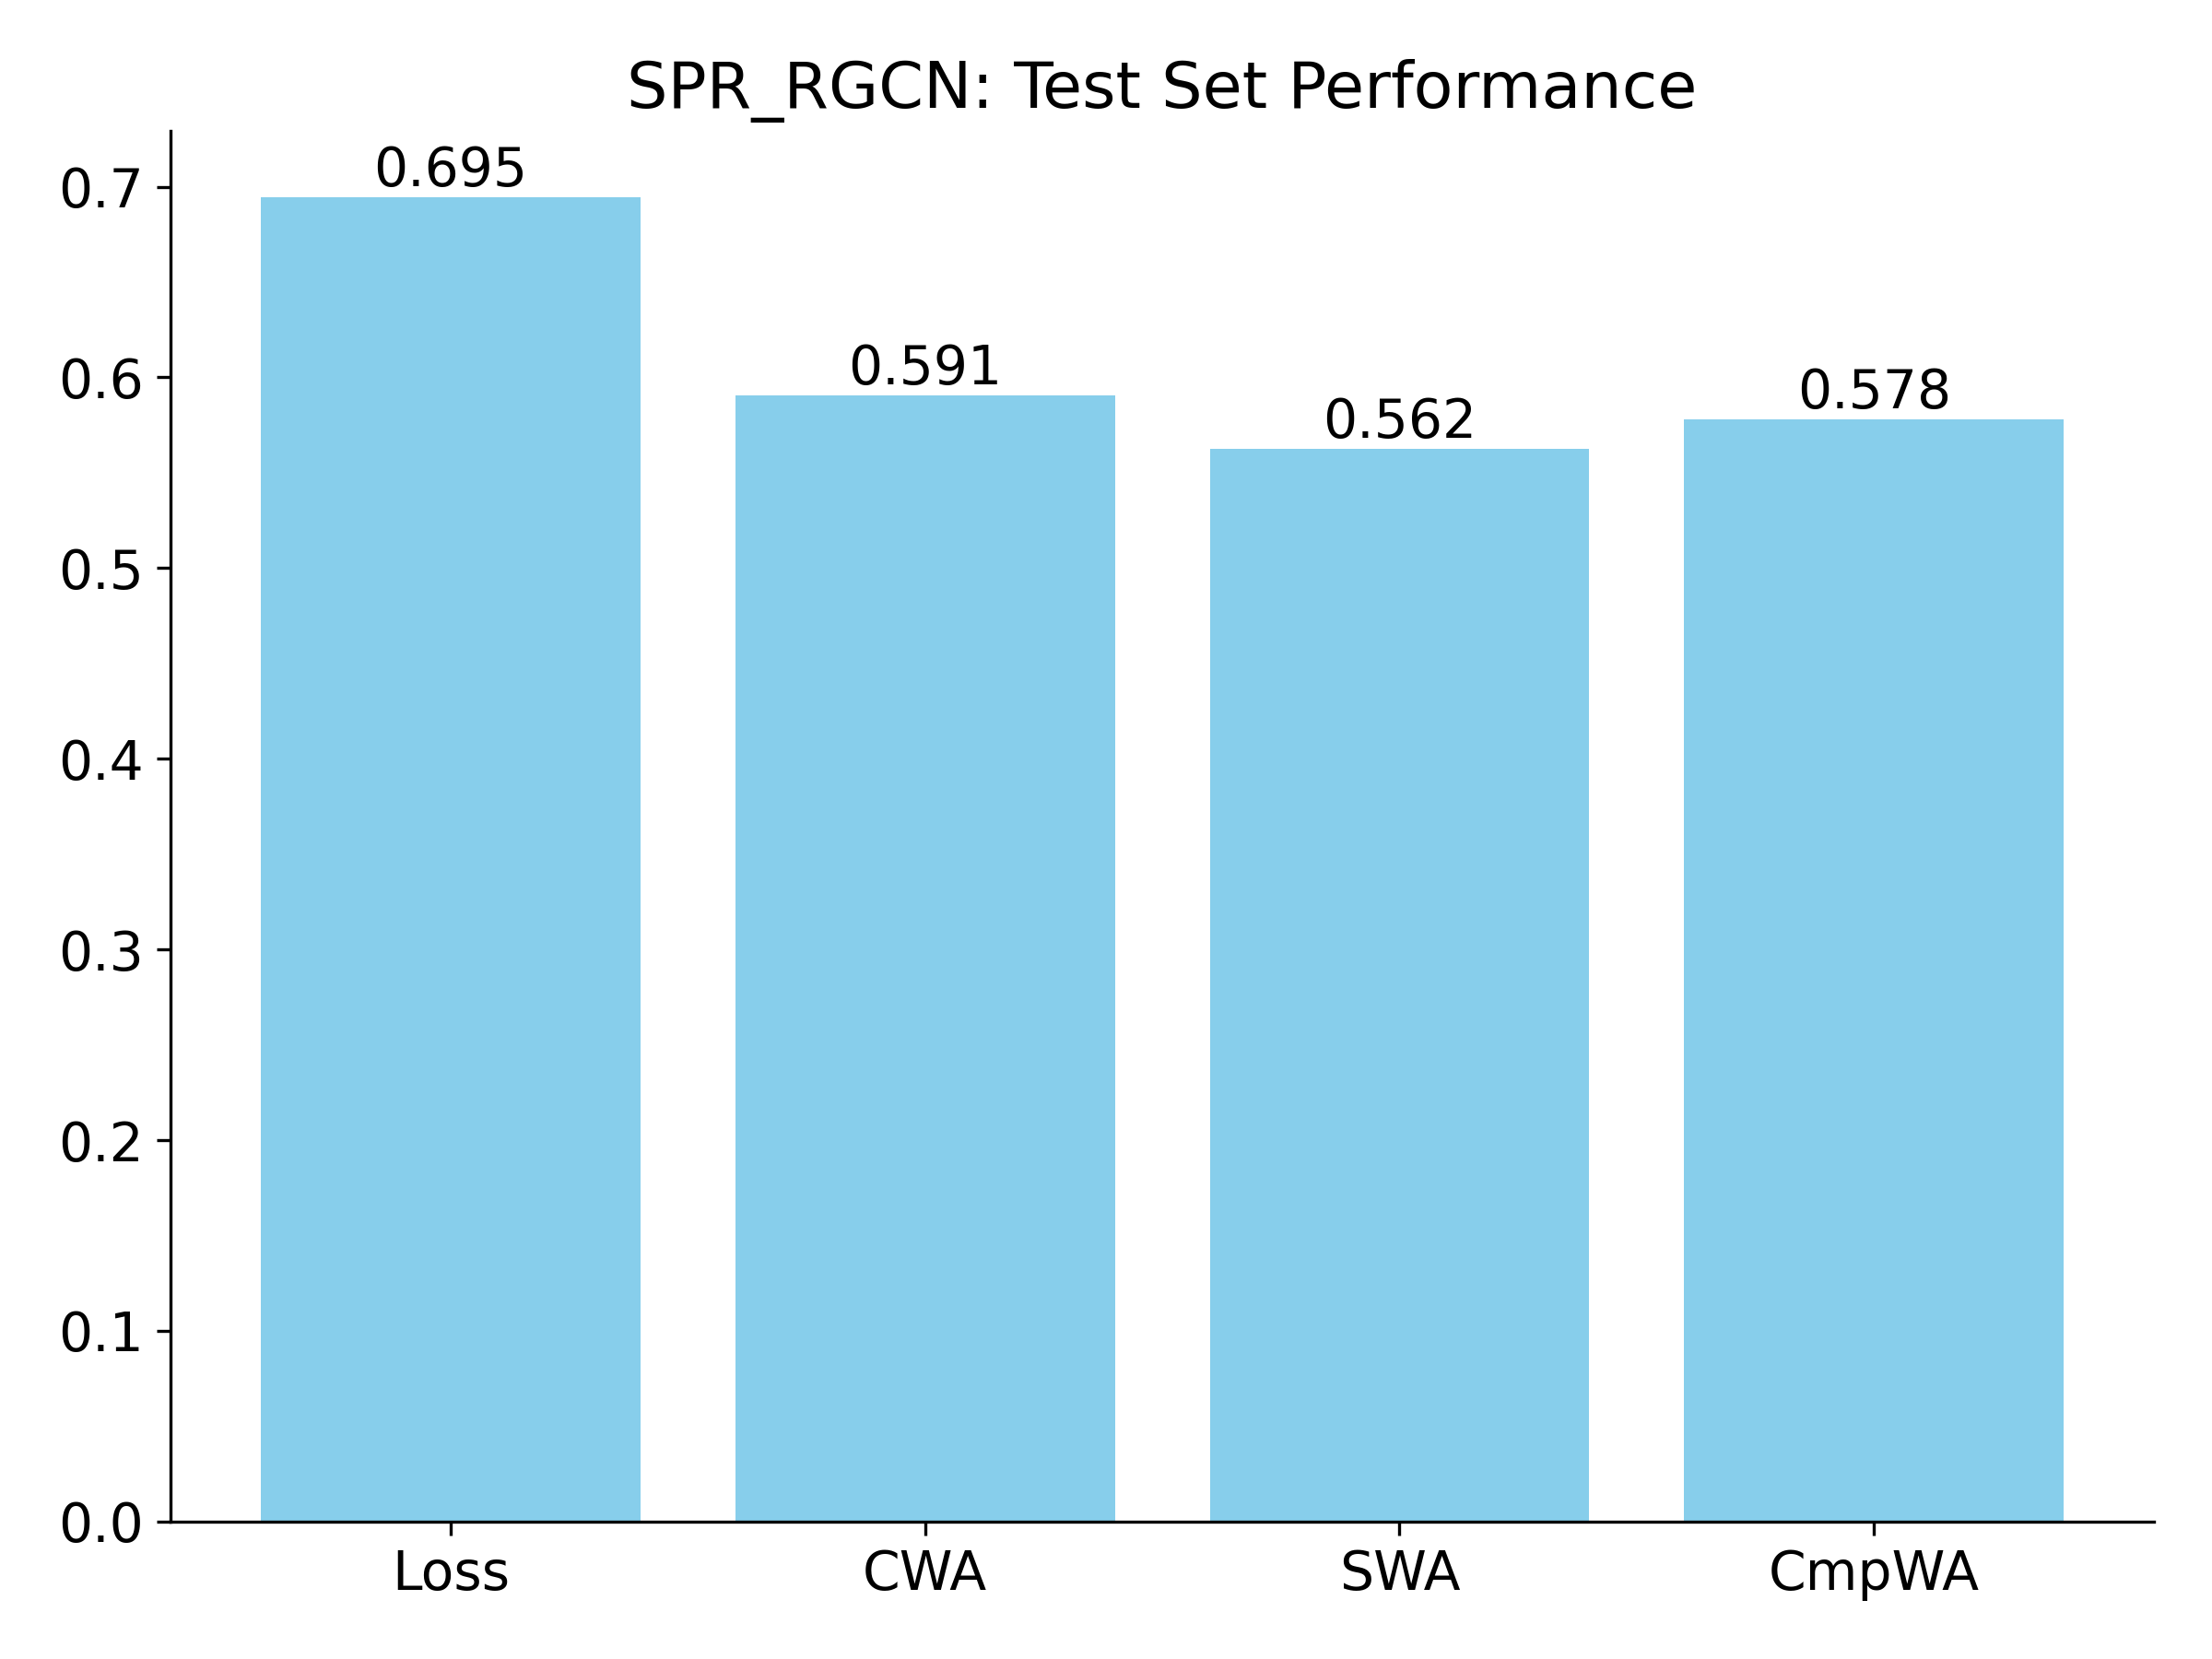
\includegraphics[width=0.45\textwidth]{SPR_RGCN_Test_Summary.png}
}
\caption{Deeper R-GCN attempts. We observe intensified overfitting and modest or no real gains in terms of final test set performance.}
\label{fig:rgcn}
\end{figure}

Although each architecture trains smoothly for a time, we do not see robust generalization. Neither additional layers nor added relational features yield consistent improvements. We believe that further research on specialized regularization or architectural constraints is needed to fully unlock deeper GNN benefits.

\section{Conclusion}
We detailed experiments showing how deeper GCNs and R-GCNs can fail to generalize, offering warnings to practitioners looking to deploy large-scale GNNs. Future work may involve new normalization strategies, domain-specific pretraining, or stronger regularization. Our findings underscore that deeper does not necessarily mean better and that more open reporting of negative results can benefit the community.

\clearpage
\bibliographystyle{plainnat}
\bibliography{references}

\appendix
\section{Additional Experiments and Visualizations}
We place supplementary results here for completeness. Some tasks do benefit slightly from deeper representations, but the overall improvements remain inconsistent. Figure~\ref{fig:multi_synthetic} shows performance on synthetic expansions. Figures~\ref{fig:no_seq_edge}, \ref{fig:multi_metric}, and \ref{fig:shallow_ablation} illustrate ablation studies and additional diagnostic plots that did not fit in the main paper.

\begin{figure}[h]
\centering
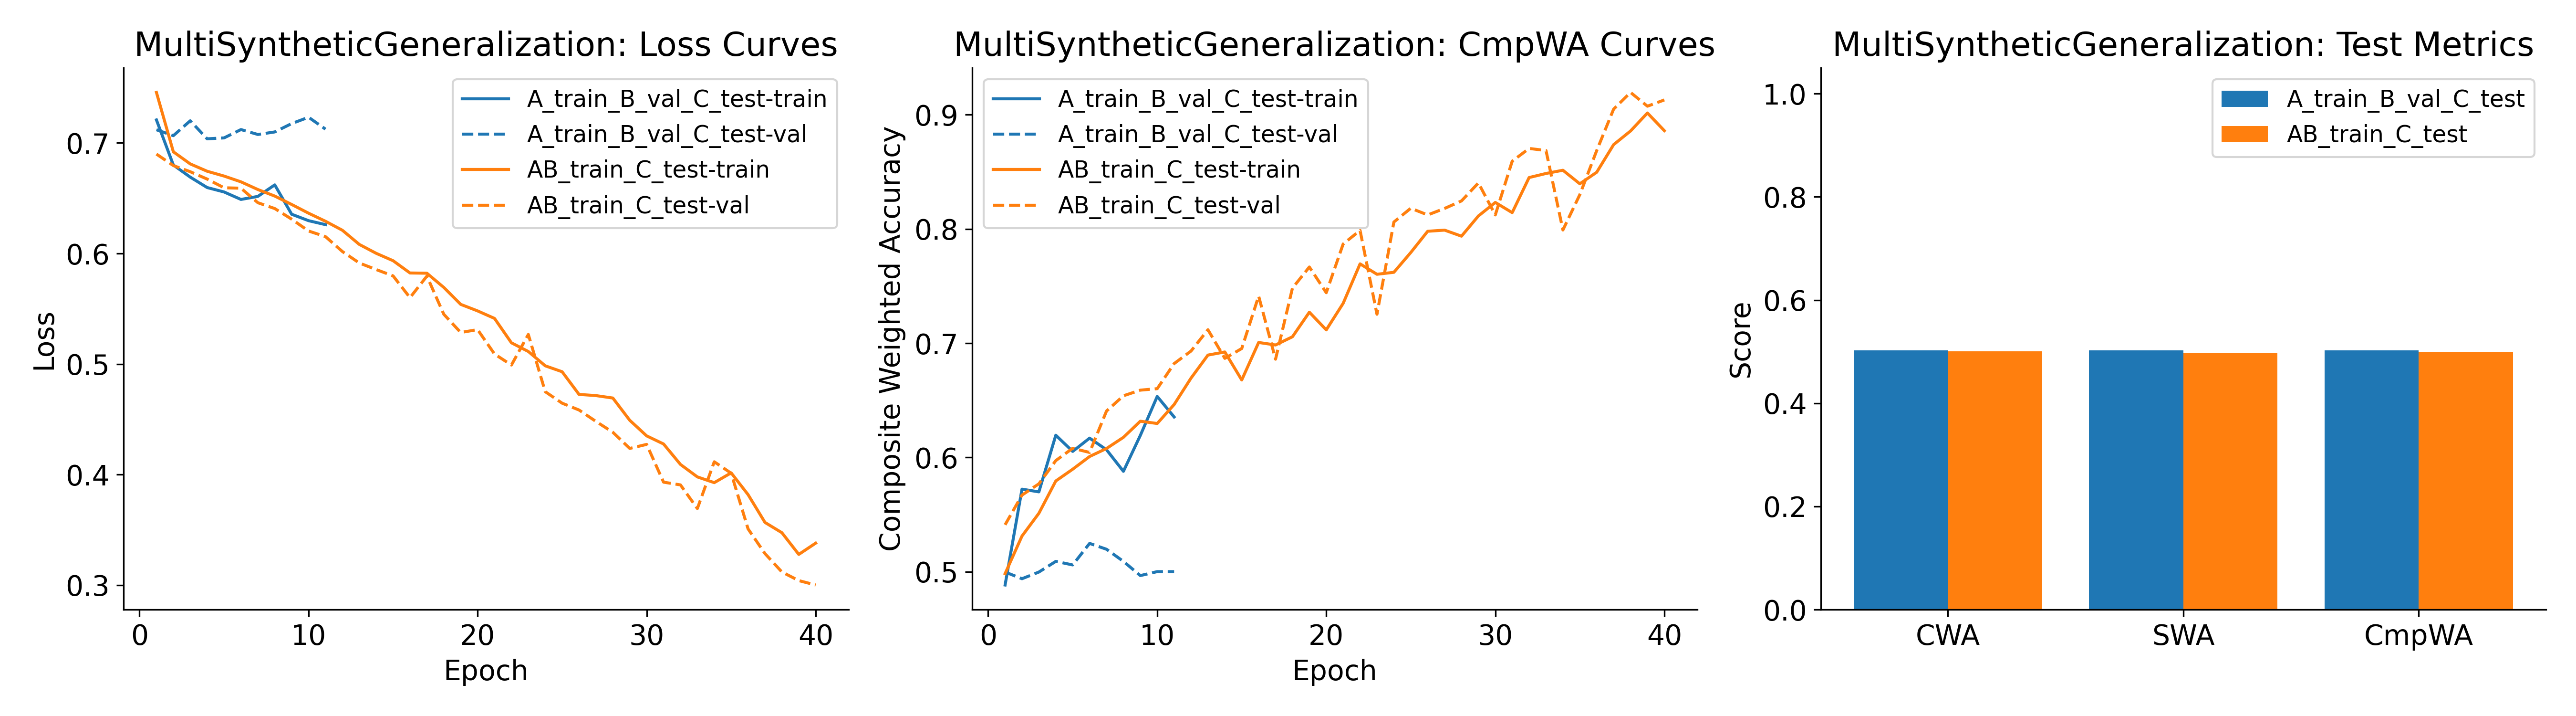
\includegraphics[width=0.45\textwidth]{MultiSyntheticGeneralization.png}
\caption{Performance across multiple synthetic expansions.}
\label{fig:multi_synthetic}
\end{figure}

\begin{figure}[h]
\centering
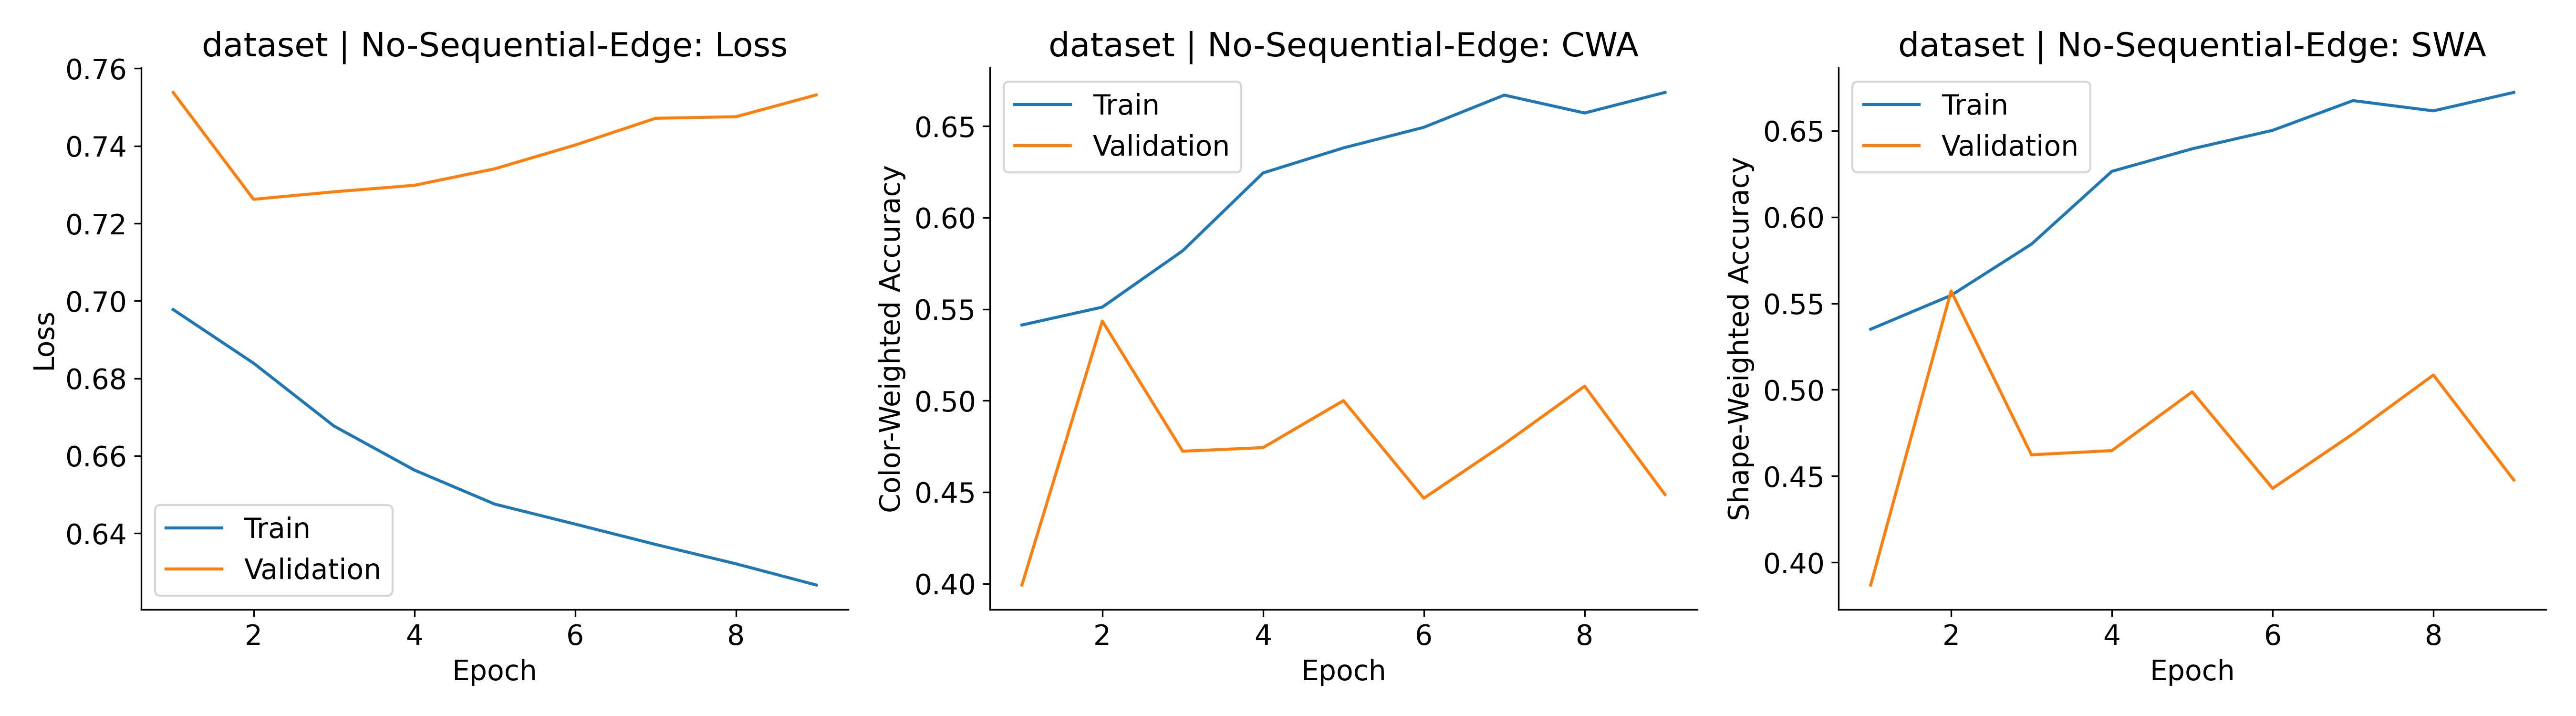
\includegraphics[width=0.45\textwidth]{NoSequentialEdge_Graph_Final.png}
\caption{Removing sequential edges.}
\label{fig:no_seq_edge}
\end{figure}

\begin{figure}[h]
\centering
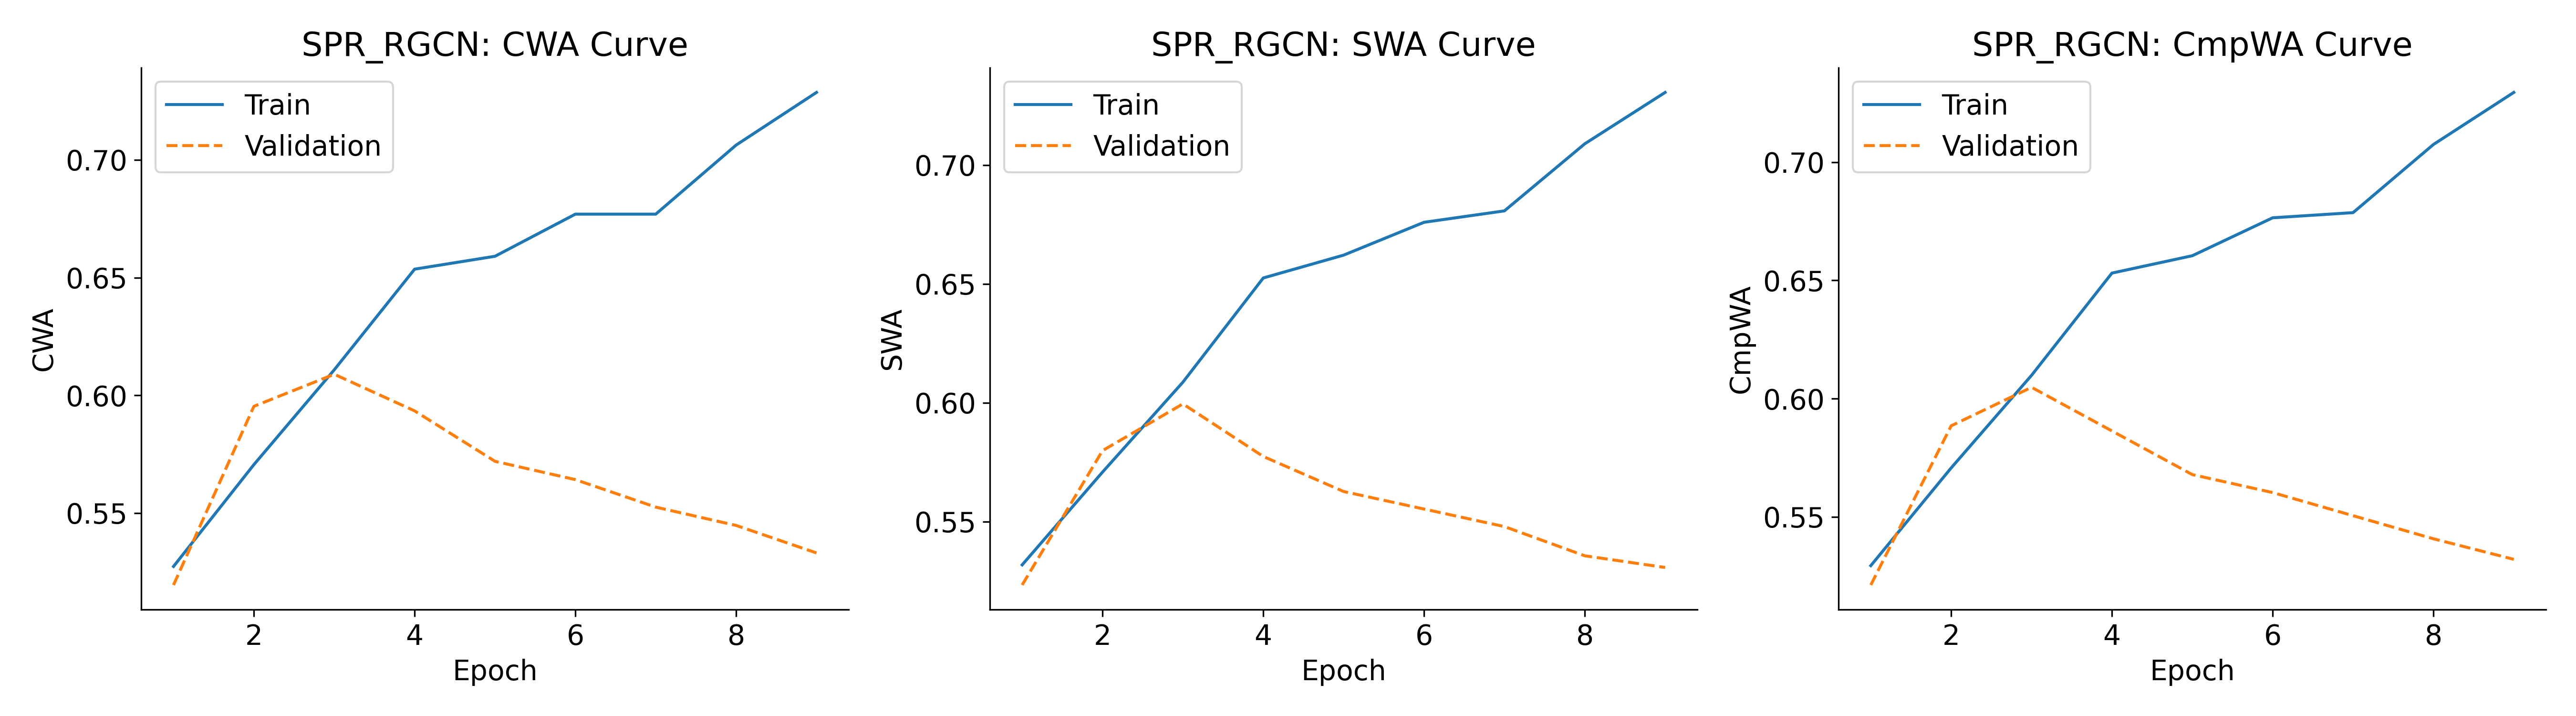
\includegraphics[width=0.45\textwidth]{SPR_RGCN_MultiMetric_Curves.png}
\caption{Detailed R-GCN performance curves across multiple metrics.}
\label{fig:multi_metric}
\end{figure}

\begin{figure}[h]
\centering
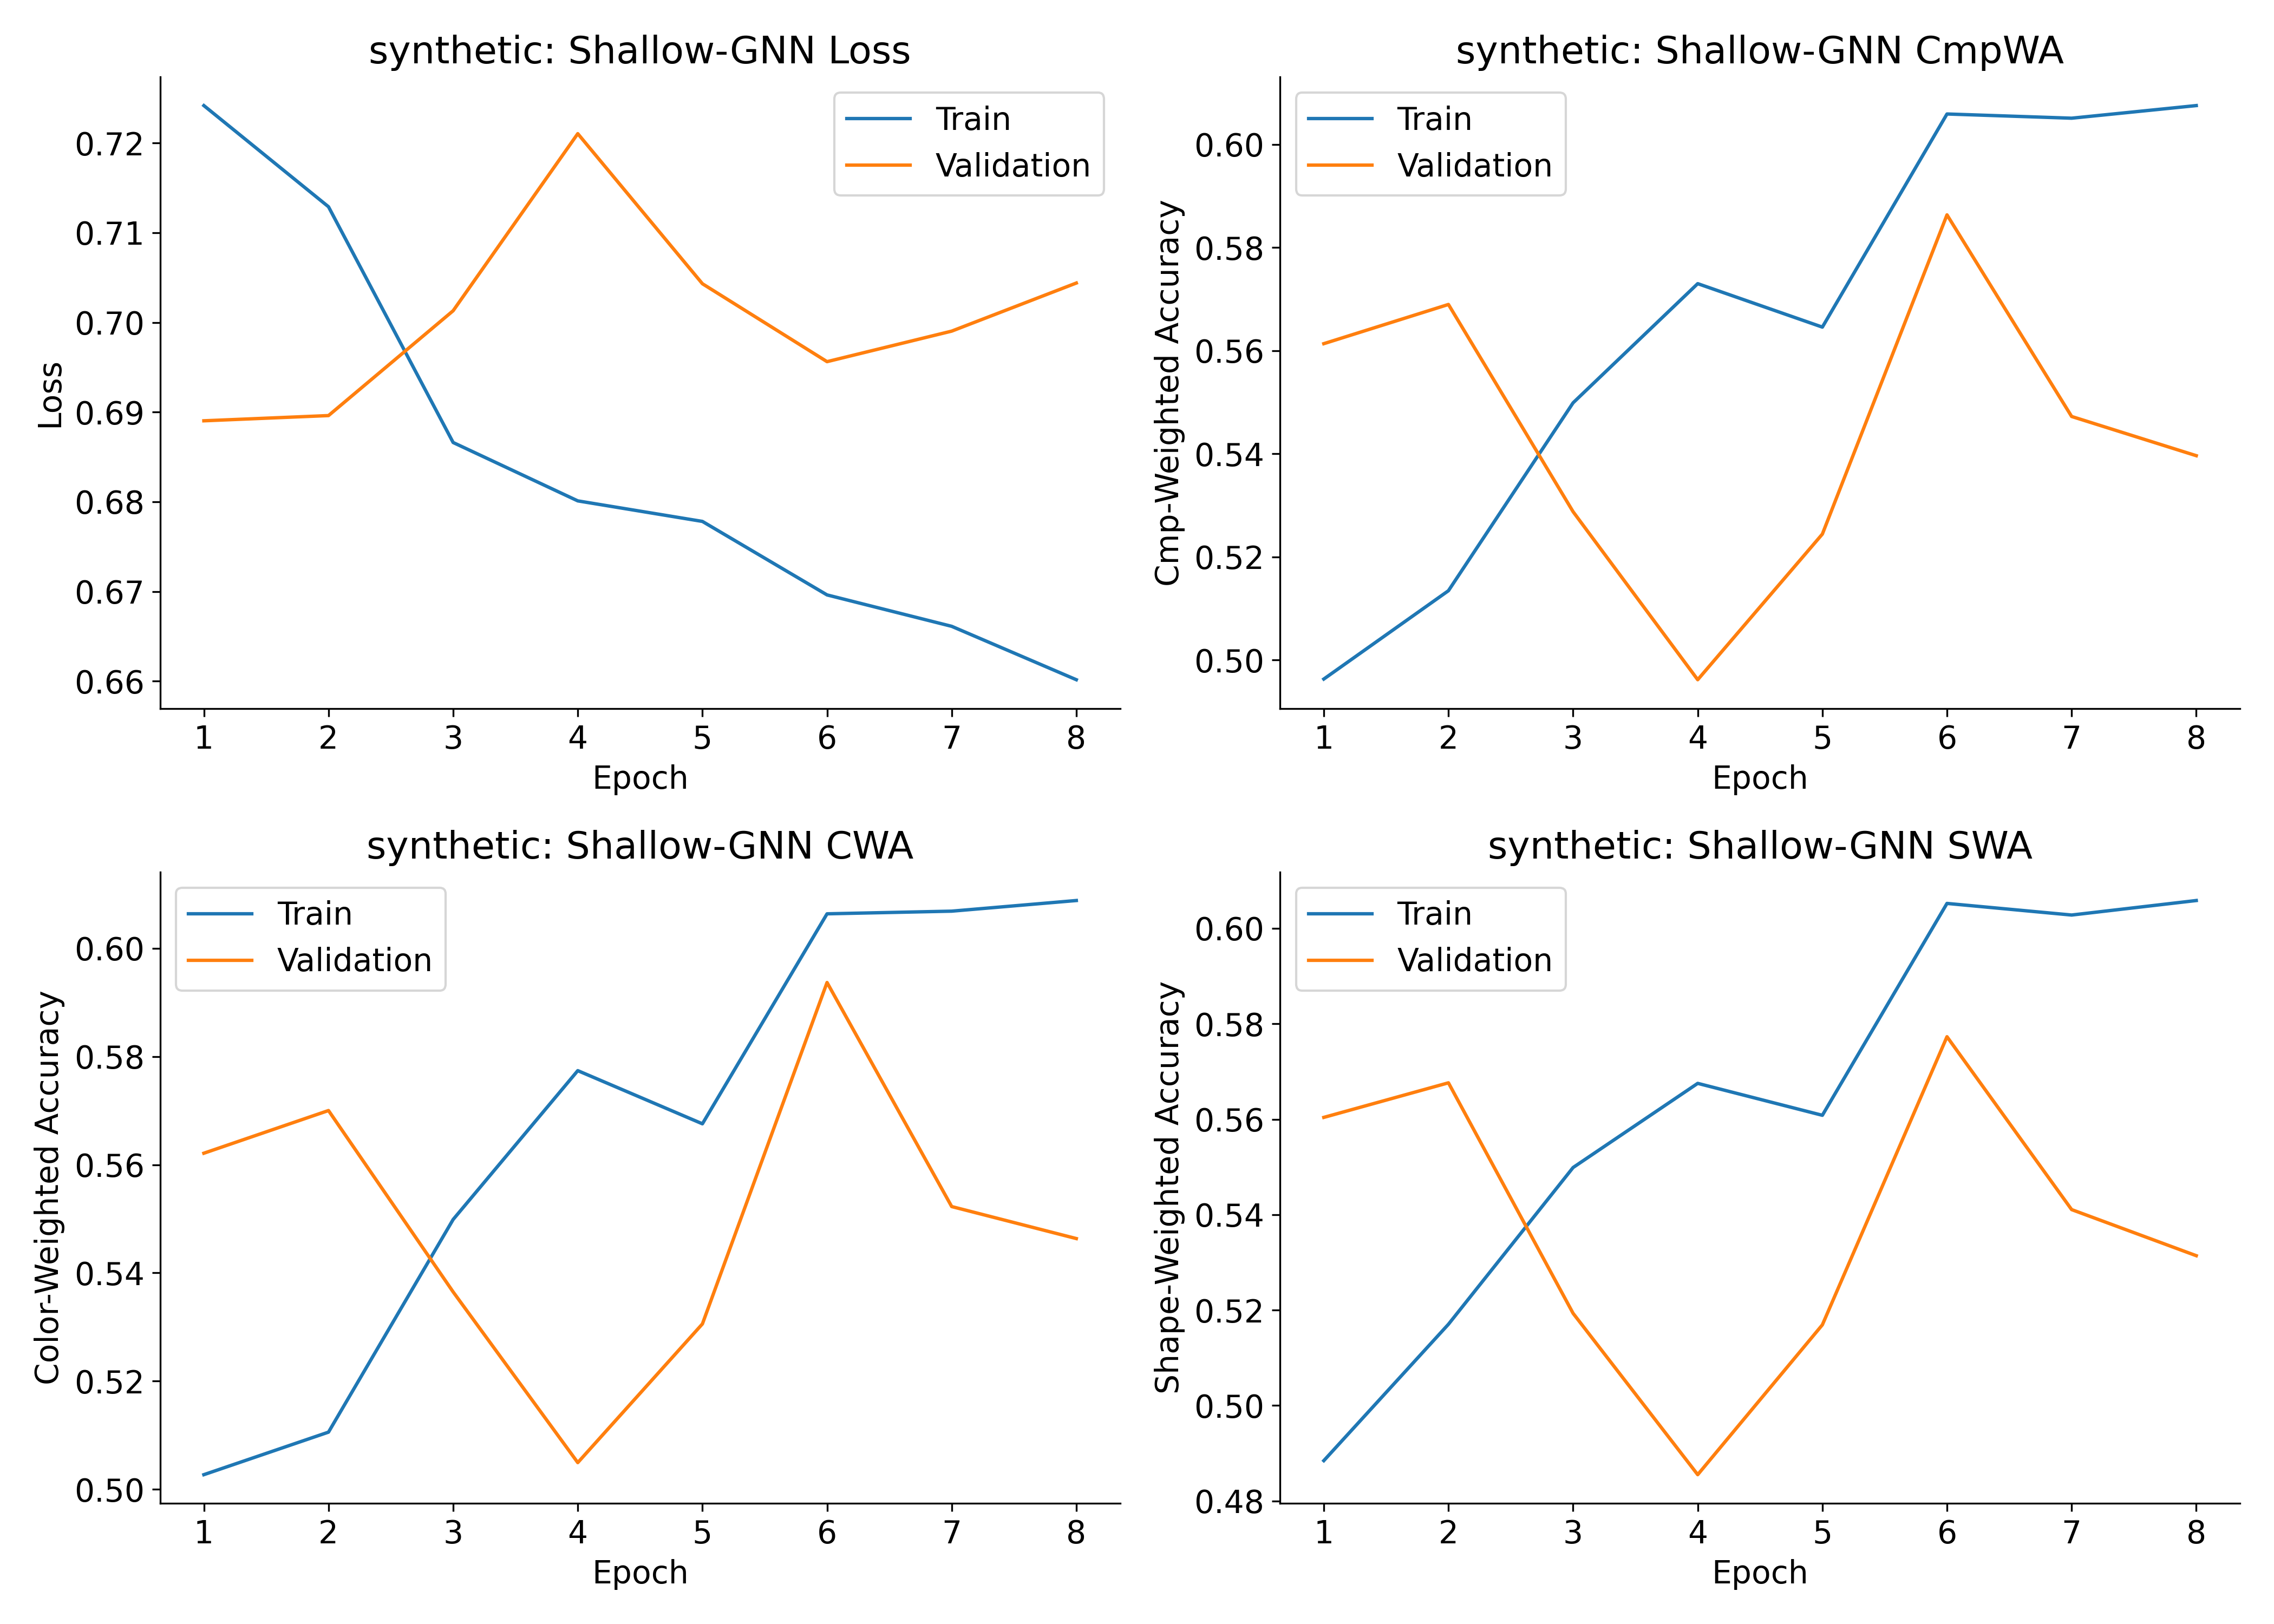
\includegraphics[width=0.45\textwidth]{ShallowGNN_Ablation.png}
\caption{Very shallow GNN ablations underfit, highlighting depth importance.}
\label{fig:shallow_ablation}
\end{figure}

\end{document}